\chapter{Getting Started}

This chapter gives you a quick overview of running QGIS and examining data available on the QGIS web page.


\section{Installation}
\index{installation}
Installation of QGIS is documented in Appendix \ref{install_guide}. The Installation Guide is distributed with the QGIS source code and is also available at \url{http://qgis.org}. Under Windows and Mac OSX, QGIS is available as a standard installer package for these platforms.


\section{Sample Data}
\index{data!sample}
If you do not have any GIS data handy, you can obtain a dataset for Alaska from the QGIS web site at \url{http://qgis.org}. The Alaska data set will be used as the basis for many of the examples and screenshots provided in this document.


\section{Starting QGIS}

Assuming that QGIS is installed in the PATH, you can start QGIS by
typing: \textbf{qgis}  at a command prompt or by double clicking on the QGIS application link (or shortcut) on the desktop. Under MS Windows, start QGIS using the Start menu shortcut, and under Mac OSX, double click the icon in your applications folder.
%\begin{figure}
%\caption{QGIS Main Window}
%\end{figure} 
\subsection{Command Line Options}\index{command line options}
QGIS supports a number of options when started from the command line. To get a
list of the options, enter \texttt{qgis ---help} on the command line. The usage
statement for QGIS is:
\small
\begin{verbatim}
Usage: /home/gsherman/qgis06_rc/bin/qgis [options] [FILES]
  options:
        [--snapshot filename]   emit snapshot of loaded datasets to given file
        [--lang language]       use language for interface text
        [--project projectfile] load the given QGIS project
        [--help]                this text
  FILES:
    Files specified on the command line can include rasters,
    vectors, and QGIS project files (.qgs):
     1. Rasters - Supported formats include GeoTiff, DEM
        and others supported by GDAL
     2. Vectors - Supported formats include ESRI Shapefiles
        and others supported by OGR and PostgreSQL layers using
        the PostGIS extension

\end{verbatim}
\normalsize
\begin{Tip} \caption{\textsc{Example Using command line arguments}}
\qgistip{
You can start QGIS by specifying one or more data files
on the command line. For example, assuming you are in your data directory,
you could start QGIS with two shapefiles and a raster file set to
load on startup using the following command: 
\ttfamily{	qgis ak\_shade.tif alaska.shp majrivers.shp}
}
\end{Tip}

\section{The QGIS Main Window}\index{main window}
When QGIS starts, you are presented with the main window as shown below.

\begin{figure}[h]
   \begin{center}
   \caption{Main window}\label{fig:startup}
   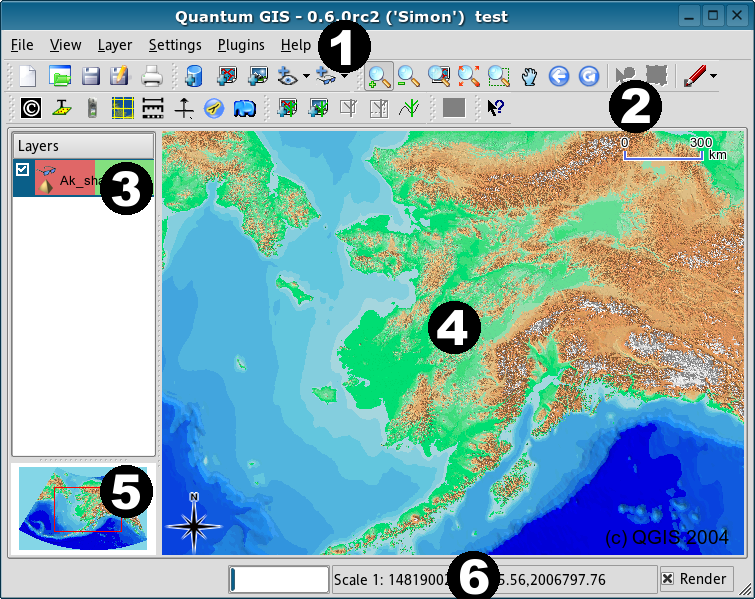
\includegraphics[scale=.5]{qgis_user_guide_images/startup}
\end{center}  
   
\end{figure}
\textsc{Note - Your window decorations (title bar, etc.) may appear different depending on your operating system and window manager}
The QGIS main window is divided into five areas:
\begin{compactenum}
\item The menu bar
\item The tool bar
\item The map legend
\item The map view
\item The map overview
\item The status bar
\end{compactenum}

These six components of the QGIS interface are described in more detail in the following sections
\subsection{The QGIS menu bar}
\index{menus}
The menu bar provides access to various QGIS features using a standard windows
heirachical menu. The top-level menus and a summary of some of the functions provided are:
\begin{compactitem}
\item File (project open, save, export image, properties)
\item Layer (add, show, hide layers)
\item View (zoom, refresh)
\item Tools (plugin manager, preferences)
\item Plugins (menus added by plugins as they are loaded)
\item Help (documentation and web links)
\end{compactitem}
%See Appendix \ref{app_menu} for complete descriptions of the menu items.

\subsection{Toolbars}
\index{toolbars}
The toolbars provide access to most of the same functions as the menus, plus
additional tools for interacting with the map. Each toolbar item has popup
help available. Hold your mouse over the item and a short description of the
tool's purpose will be displayed. %See Appendix \ref{app_toolbar} for complete
%descriptions and illustrations of the various toolbars.  

\subsection{The QGIS map legend}
\index{legend}
The map legend area is used to set the visibility and z-ordering of layers.
Z-ordering means that layers listed nearer the top of the legend are drawn
over layers listed lower down in the legend. The checkbox in each legend entry
can be used to show/hide that layer.\index{layer!visibility}
\begin{Tip} \caption{\textsc{Viewing the Layer Menu}}\index{layer!context menu}
\qgistip{You can display the context menu for any layer in the legend by right-clicking
on the layer name. The context menu contains items for working with the layer and viewing
its properties.}
\end{Tip}

Each legend entry can show the following mini icons:


\includegraphics[scale=1]{qgis_user_guide_images/pyramid} This is a raster layer that has pyramids built for it to improve rendering efficiency (see Section \ref{raster_pyramids}).\\
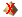
\includegraphics[scale=1]{qgis_user_guide_images/no_pyramid} This is a raster that has no pyramid layers (see Section \ref{raster_pyramids}).\\

\includegraphics[scale=1]{qgis_user_guide_images/inoverview} This layer is shown in the overview map area as well as in the main map window.\\

\includegraphics[scale=1]{qgis_user_guide_images/editable} This is a vector layer that is currently enabled for editing.\\
\subsection{The QGIS map view}
\index{map!view}
This is the 'business end' of QGIS - maps are displayed in this area! The map
displayed in this window will depend on the vector and raster layers you have
chosen to load (see sections that follow for more info on this). The map view
can be panned (shifting to focus of the map display to another region), zoomed
in and out, and supports various other actions as described in the toolbar
description above.  The map view and the legend are tightly bound to each
other - the maps in view reflect changes you make in the legend area.  
\begin{Tip}\caption{\textsc{Zooming the Map with the Mouse
Wheel}}\index{zoom!mouse wheel}
\qgistip{You can use the mouse wheel to zoom in and out on the map. Place the mouse cursor inside the map area and roll it forward (away from you) to zoom in and backwards (towards you) to zoom out.
}
\end{Tip}
\subsection{The QGIS map overview}
\index{map!overview}
The map overview area provides a full extent view of layers added to it. Within the view is a rectangle showing the current map extent. This allows you to quickly determine which area of the map you are currently viewing. Note that labels are not rendered to the map overview even if the layers in the map overview have been set up for labelling.

\subsection{The QGIS map status bar} 
The status bar shows you your current position in map coordinate (e.g. meters
or decimal degress) as the mouse pointer is moved accross the map view. The status bar also shows the view extents of the map view as you pand and zoom in and out. A progress bar in the status bar shows progress of rendering as each layer is drawn to the map view. In some cases such as the gathering of statistics in raster layers, the progress bar will be used to show the status of lengthy operations. At the end of the status bar is a small checkbox which can be used to temporarily prevent layers being rendered to the map view )see Section \ref{subsec:redraw_events} below.

\section{Rendering}\label{subsec:redraw_events}\index{rendering}
By default, QGIS renders all visible layers whenever the map canvas must be refreshed. The events that trigger a refresh of the map canvas include:
\begin{compactitem}
\item Adding a layer
\item Panning or zooming
\item Resizing the QGIS window
\item Changing the visibility of a layer or layers
\end{compactitem}
QGIS allows you to control the rendering process in a number of ways.

\subsection{Scale Dependent Rendering}\index{rendering!scale dependent}
Scale dependent rendering allows you to specify the minimum and maximum scales
at which a layer will be visible.  To set scale dependency rendering, open the
properties dialog by double-clicking on the layer in the legend. On the
\textit{General} tab, set the minimum and maximum scale values and then click on
the \textit{Use scale dependent rendering} checkbox.

You can determine the scale values by first zooming to the level you want to use
an noting the scale value in the QGIS status bar.\index{scale}
\subsection{Controlling Map Rendering}
Map rendering can be controlled in the following ways:
\begin{compactenum}
\item Stopping rendering during drawing of the map canvas
\item Temporarily suspending rendering
\item Setting an option to control the visibility of layers when they are added
\end{compactenum}
\subsection{Stopping Rendering}\index{rendering!halting}
To stop the map drawing, press the ESC key. This will halt the refresh of the
map canvas and leave the map partially drawn. It may take a bit of time between
pressing ESC and the time the map drawing is halted.
\subsection{Suspending Rendering}\index{rendering!suspending}
To suspend rendering, click the \textit{Render} checkbox in the lower right
corner of the statusbar. When the \textit{Render} box is not checked, QGIS does
not redraw the canvas in response to any of the events described in Section
\ref{sec:redraw_events}. Examples of when you might want to suspend rendering
include:
\begin{compactitem}
\item Add many layers and symbolize them prior to drawing
\item Add one or more large layers and set scale dependency before drawing
\item Add one or more large layers and zoom to a specific view before drawing
\item Any combination of the above
\end{compactitem}
Checking the \textit{Render} box enables rendering and causes and immediate
refresh of the map canvas.
\subsection{Setting Layer Add
Option}\index{rendering!options}\index{layers!initial visibility}
You can set an option to always load new layers without drawing them. This means
the layer will be added to the map, but its visibility checkbox in the legend
will be unchecked by default. To set this option, choose \textit{Preferences} from the
\textit{Settings} menu and click on the \textit{Rendering} tab. Check the
\textit{New layers added to the map are not displayed} checkbox. Any layer added
to the map will be off (invisible) by default.
\subsection{Updating the Map Display During Rendering}\index{rendering!update
during drawing}
You can set an option to update the map display as features are drawn. By
default, QGIS does not display any features for a layer until the entire layer
has been rendered. To update the display as features are read from the
datastore, choose \textit{Preferences} from the
\textit{Settings} menu and click on the \textit{Rendering} tab. Set the feature
count to an appropriate value to update the display during rendering. Setting a
value of 0 disables update during drawing (this is the default). Setting a value
too low will result in poor performance as the map canvas is continually updated
during the reading of the features. A suggested value to start with is 500. 

